% Simple pipeline figure (standalone: compile with pdflatex, or copy the tikzpicture into paper.tex)
\documentclass[border=6pt]{standalone}
\usepackage{tikz}
\usetikzlibrary{positioning,arrows.meta,calc}
\definecolor{head}{HTML}{1F4E9E}      % block headings
\definecolor{ex}{HTML}{4A4A4A}        % example text
\newcommand{\hd}[1]{{\large\bfseries\color{head}#1}}
\newcommand{\ex}[1]{{\normalsize\color{ex}#1}}
\hyphenpenalty=10000 \exhyphenpenalty=10000
\begin{document}
\begin{tikzpicture}[
    box/.style={draw, rounded corners=3pt, thick, minimum width=4cm, minimum height=2.2cm,
                text width=3.9cm, align=center, fill=white},
    llm/.style={box, fill=blue!8},
    res/.style={box, fill=green!10},
    imgbox/.style={draw, rounded corners=3pt, thick, align=center, fill=white, inner sep=5pt},
    note/.style={font=\normalsize, text=black!70},
    arrow/.style={->, >=Stealth, very thick}
]
\node[imgbox] (map) at (0,2.2) {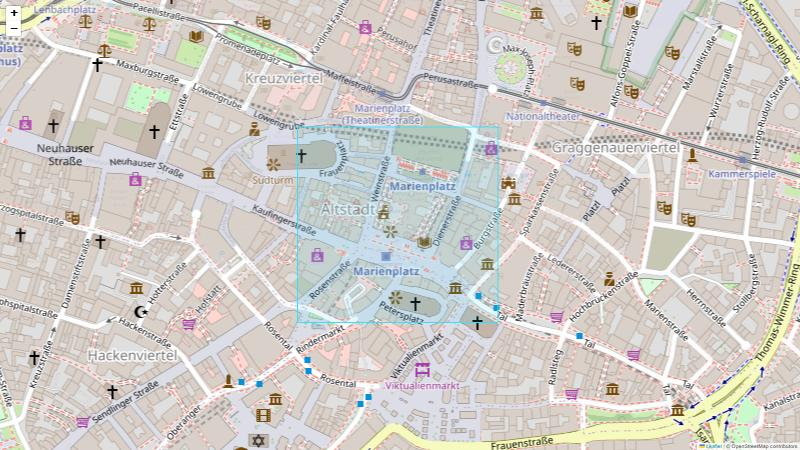
\includegraphics[width=5.2cm]{images/map_bbox.jpg}\\[3pt]\hd{Map area}\\[1pt]\ex{bbox: 48.1362, 11.5735, 48.1390, 11.5778}};
\node[box] (prompt) at (0,-2.6) {\hd{Text prompt}\\[2pt]\ex{``Walk along the sidewalk to the bus stop''}};
\node[box] (model) at (6.6,0) {\hd{Map context}\\[2pt]\ex{roads, crossings, signals, benches\ldots}};
\node[llm] (rules) at (12.2,2) {\hd{1. Task rules}\\[2pt]\ex{what the ego pedestrian must do}};
\node[llm] (world) at (12.2,-2) {\hd{2. Scene}\\[2pt]\ex{cars, lights, start point}};
\node[box] (check) at (17.8,0) {\hd{Checker}\\[2pt]\ex{does it fit the map?}};
\node[res] (file) at (23.4,0) {\hd{Scenario files}\\[2pt]\ex{OpenSCENARIO\\Python script\\OpenDRIVE road network}};
\node[imgbox, fill=green!10] (play) at (30,0) {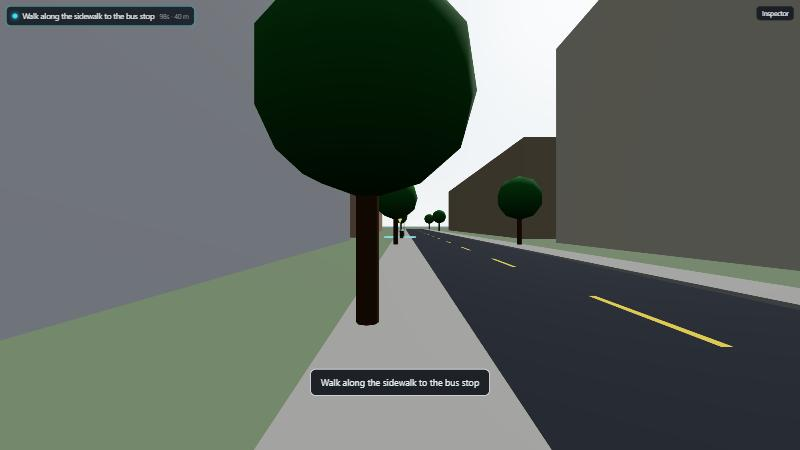
\includegraphics[width=5.2cm]{images/player_ptp.jpg}\\[3pt]\hd{Player}\\[1pt]\ex{a person walks it in VR}};

\draw[arrow] (map) -- (model);
\draw[arrow] (prompt) -- (model);
\draw[arrow] (model) -- (rules);
\draw[arrow] (model) -- (world);
\draw[arrow] (rules) -- (world);
\draw[arrow] (rules) -- (check);
\draw[arrow] (world) -- (check);
\draw[arrow] (check) -- (file);
\draw[arrow] (file) -- (play);
\draw[arrow] (check.north) -- ++(0,2.9) -| node[pos=0.25, above, note]{error} (rules.north);
\node[note] at (12.2,-4.1) {blue: written by a local language model};
\end{tikzpicture}
\end{document}
